\section{The team}\label{sec:method}

\begin{figure*}[tbp]
\centering
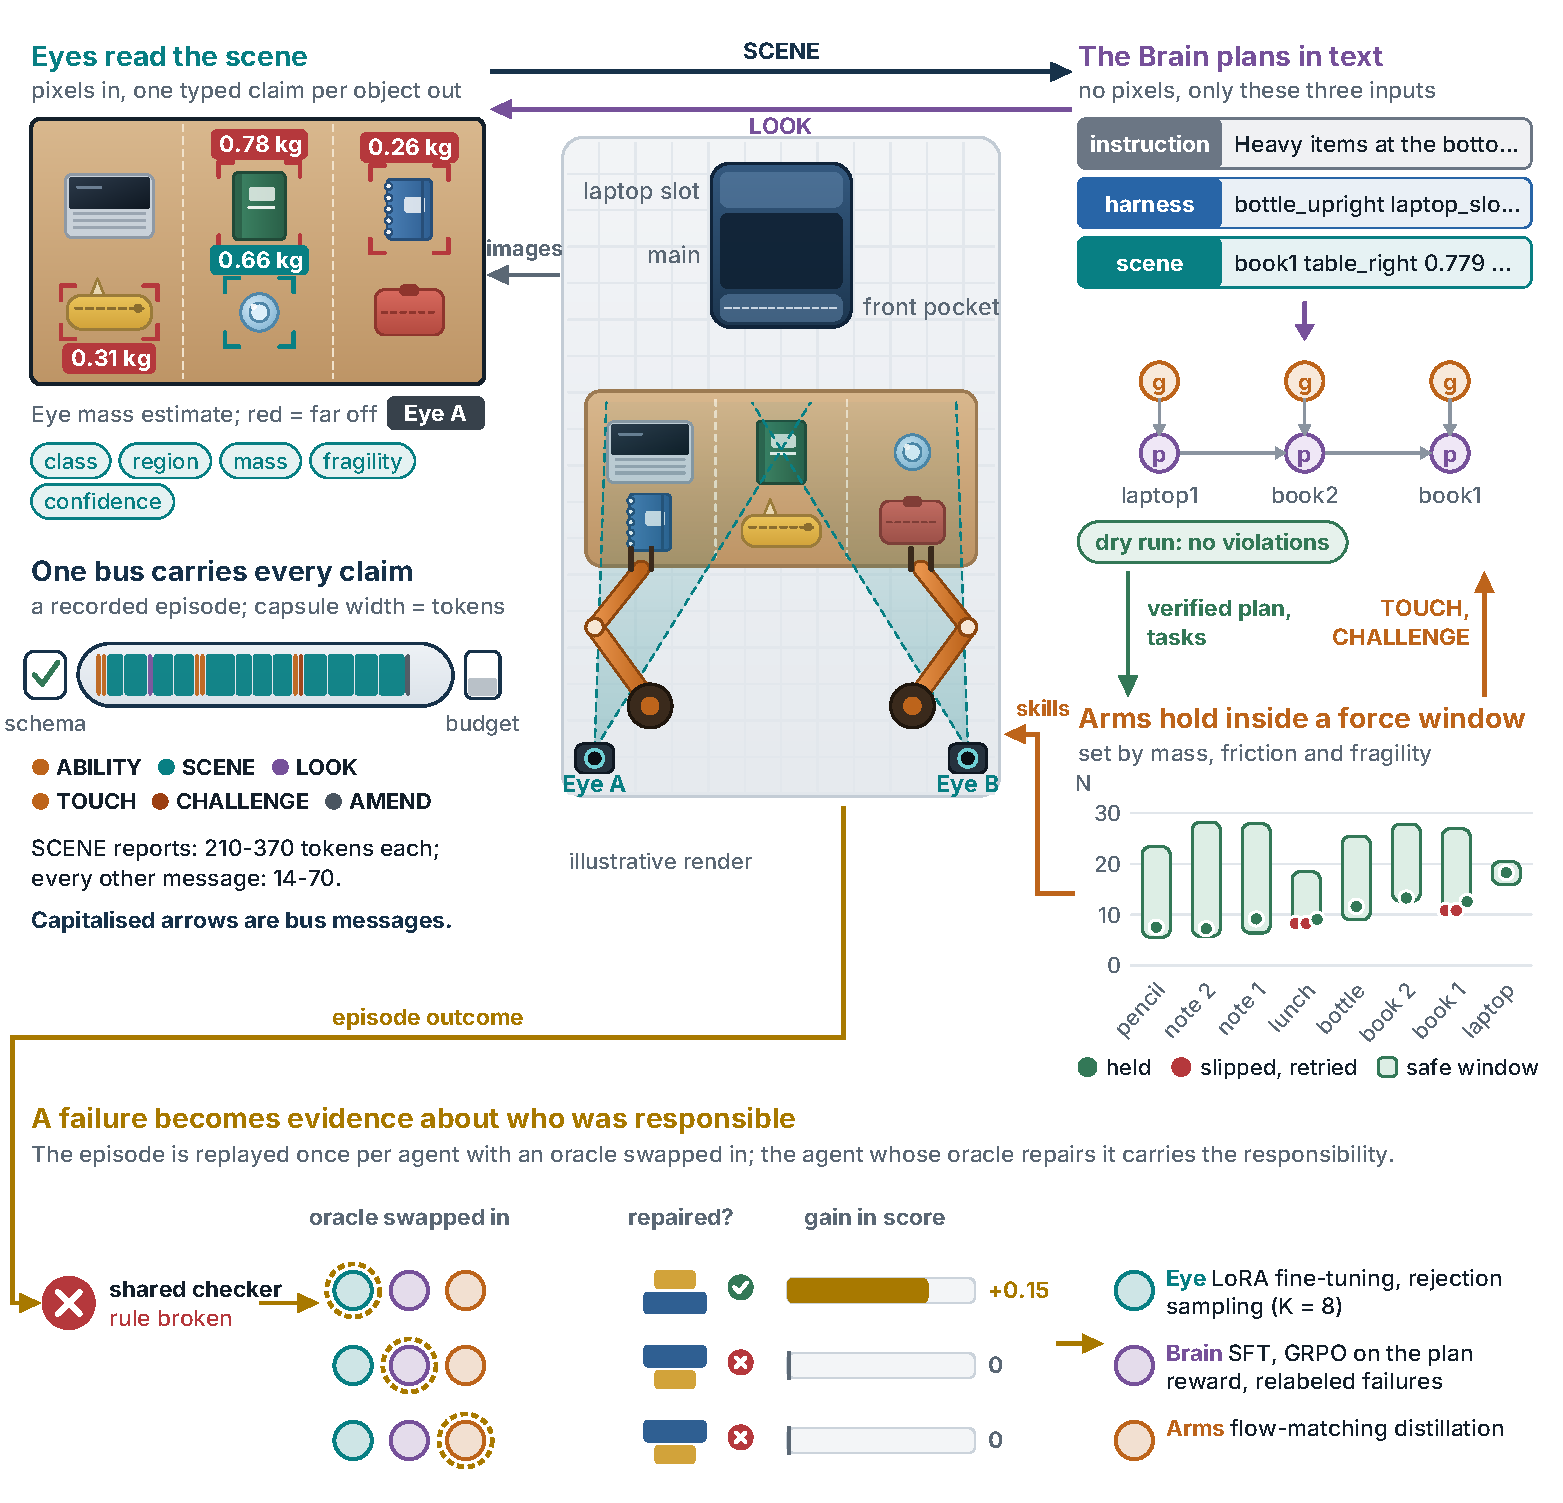
\includegraphics[width=0.92\textwidth]{fig_overview}
\caption{\textbf{The team and its interfaces.} Eyes see pixels and emit a structured scene; the Brain reads text, retrieves from the harness, and plans; a verifier checks the plan before the scheduler hands tasks to two blind Arms; touch and challenges flow back through a typed message bus. Numbers give the order of one episode. Dashed boxes are optional; red tags mark components whose trained models do not yet exist.}
\label{fig:overview}
\end{figure*}

\subsection{Task, roles and failure model}\label{sec:task}
The task is to pack a backpack from a table: given a short natural-language instruction (for example which items to pack and which rules to respect), two arms must place the requested items into the bag's compartments.
The six rules are in \cref{tab:rules}: heavier items go first so that they sit at the bottom of the main compartment, the laptop goes in its slot, the bottle stays upright and apart from the laptop, the lunchbox goes in last, distractor items are left alone, and only one arm may be at the bag at a time.
The team has three kinds of agents (\cref{fig:overview}).
Each \emph{Eye} is a vision-language model that sees an image and emits a JSON scene listing each object's class, region, estimated mass and fragility.
The \emph{Brain} is a text-only language model; it never sees pixels and plans a directed acyclic graph of grasp and place tasks.
Each \emph{Arm} is blind: it has proprioception, force sensing and a skill interface, and reports what it feels.
Failures are charged to an agent by the loop's attribution rules (\cref{sec:success}); these are heuristic labels, which we validate in \cref{sec:experiments}.

\begin{table}[tbp]
\centering\small
\begin{tabular}{lp{0.74\linewidth}}
\toprule
Rule file & Text given to the Brain (verbatim from the harness file) \\
\midrule
\texttt{bag\_exclusive} & Only one arm may place into the bag at a time. Serialize place tasks with dependencies. \\
\texttt{bottle\_upright} & Water bottles go in upright and in a different compartment from the laptop. Use orientation=upright. \\
\texttt{heavy\_bottom} & Place heavier items first so they sit at the bottom of the main compartment; lighter items go on top. Sort items by estimated mass, descending. \\
\texttt{laptop\_slot} & The laptop goes in the compartment named by the instruction (default: the padded laptop slot). Never stack other items on or beside it in the same compartment. \\
\texttt{leave\_distractors} & Items the instruction says to leave (for example the mug and the plate) must not be touched, moved or pushed aside. \\
\texttt{lunchbox\_last} & The lunchbox is packed last so it sits on top and stays accessible. \\
\bottomrule
\end{tabular}

\caption{The six rules the team must satisfy; the text is the harness file the Brain retrieves (\cref{sec:harness}).}
\label{tab:rules}
\end{table}

\subsection{Typed messages}\label{sec:bus}
Agents exchange \nMsgTypes{} message types (\cref{fig:messages}, \cref{tab:messages}): scene reports, ability declarations, task claims and offers, status and blockage notices, touch feedback, requests to look again, challenges, handovers, locks and amendments of the instruction.
The bus checks each message against its schema, charges an approximate token count (about four characters per token, a tokenizer-free proxy) and enforces a per-episode budget; an over-budget message is refused and the sender is told.
We implement four communication modes: \emph{push} sends the full scene every round, \emph{delta} sends only changed objects, \emph{pull} sends on request and after failures, and \emph{init-only} sends once.
The modes trade tokens for information, and their effect on trained agents is a pending ablation (\cref{tab:ablations}); the accounting itself is checked on the fixture in appendix~F.

\begin{figure*}[tbp]
\centering
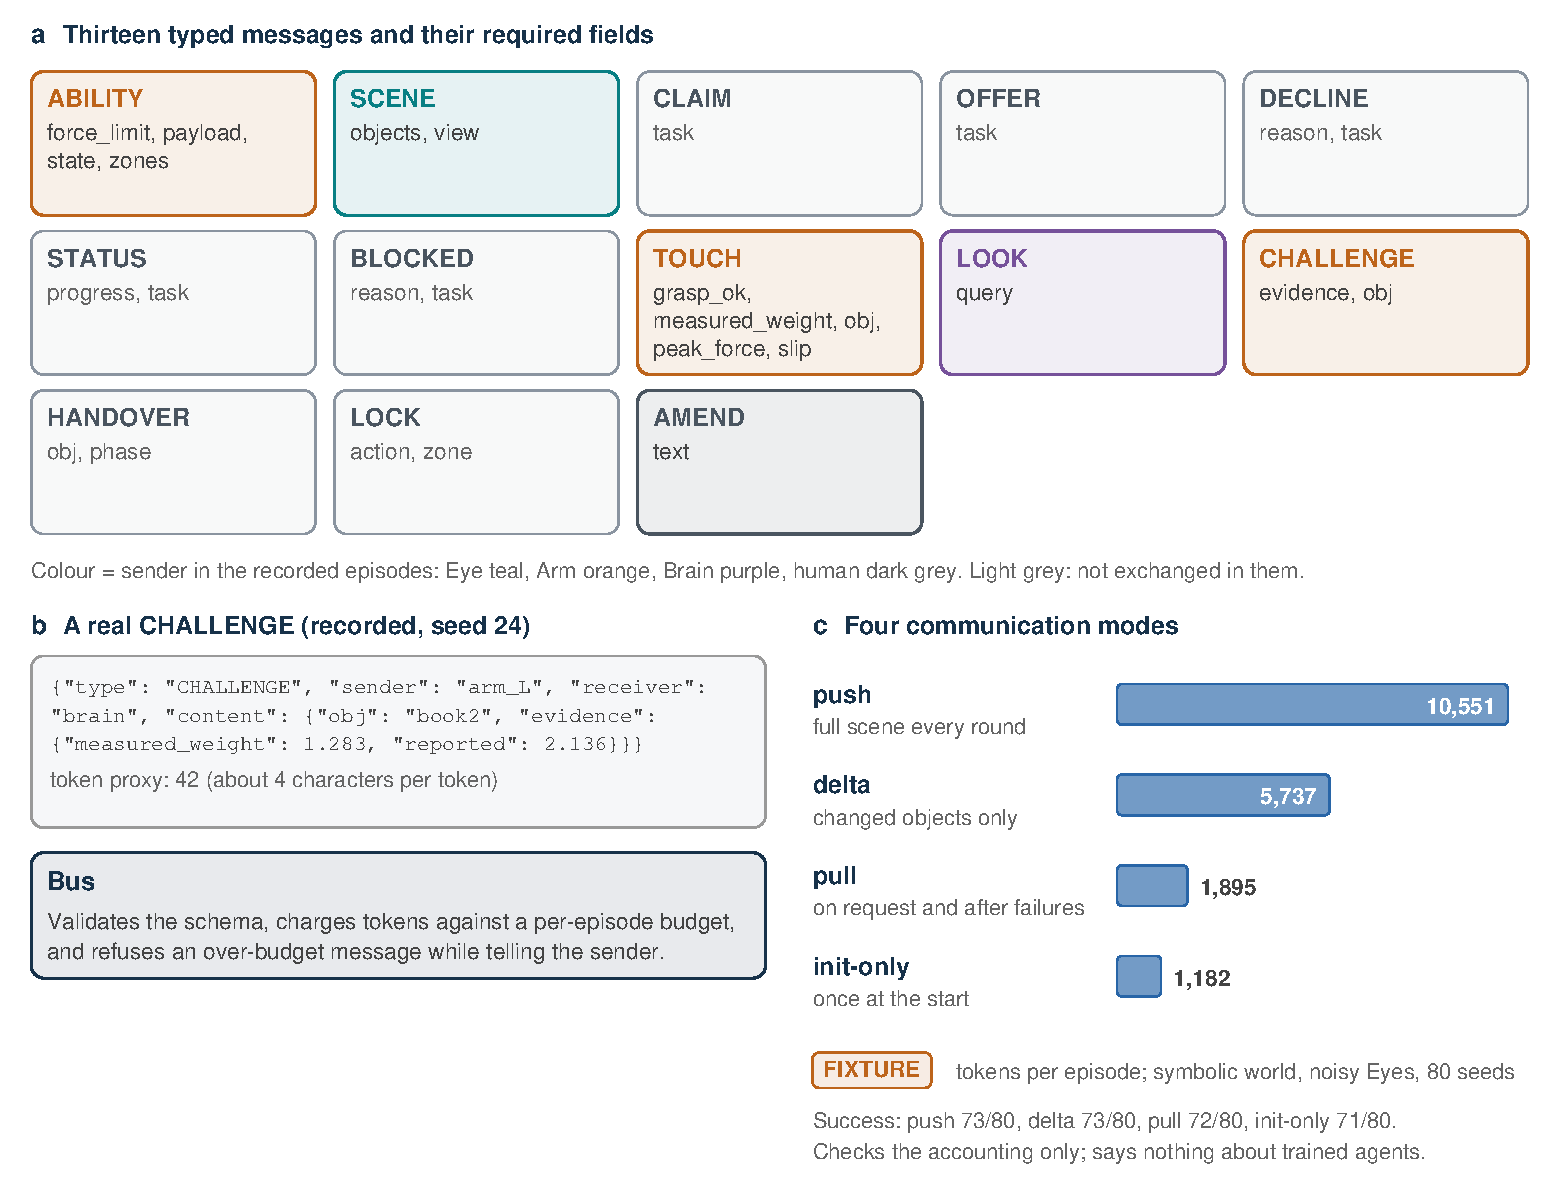
\includegraphics[width=\textwidth]{fig_messages}
\caption{\textbf{The message layer.} (a)~The \nMsgTypes{} types and their required fields; colour shows the sender observed in the recorded episodes. (b)~A recorded CHALLENGE: an Arm reports a measured weight that disagrees with the Eye's report. (c)~Message tokens per episode under four communication modes, from the symbolic fixture (80 seeds): a check that the accounting works, not a result about trained agents.}
\label{fig:messages}
\end{figure*}

\begin{table}[tbp]
\centering\scriptsize
\begin{tabular}{lp{0.38\linewidth}p{0.3\linewidth}}
\toprule
Type & Required fields & Sender in the recorded episode \\
\midrule
\texttt{ABILITY} & force\_limit, payload, state, zones & arm \\
\texttt{SCENE} & objects, view & eye \\
\texttt{CLAIM} & task & not exchanged in the recorded episode \\
\texttt{OFFER} & task & not exchanged in the recorded episode \\
\texttt{DECLINE} & reason, task & not exchanged in the recorded episode \\
\texttt{STATUS} & progress, task & not exchanged in the recorded episode \\
\texttt{BLOCKED} & reason, task & not exchanged in the recorded episode \\
\texttt{TOUCH} & grasp\_ok, measured\_weight, obj, peak\_force, slip & arm \\
\texttt{LOOK} & query & brain \\
\texttt{CHALLENGE} & evidence, obj & arm \\
\texttt{HANDOVER} & obj, phase & not exchanged in the recorded episode \\
\texttt{LOCK} & action, zone & not exchanged in the recorded episode \\
\texttt{AMEND} & text & human \\
\bottomrule
\end{tabular}

\caption{Message schema as implemented. The sender column lists what was observed in the recorded episode of \cref{fig:loop}; it is not a constraint of the schema.}
\label{tab:messages}
\end{table}

\subsection{The harness}\label{sec:harness}
The Brain's procedural knowledge lives in \nHarnessFiles{} short markdown files (\cref{fig:harness}, appendix~B): the six rules, four skill descriptions, object and agent notes, an episode memory and a task template.
Retrieval is a two-pass BM25 search.
Pass one queries with the instruction and returns the top five of the six rules; pass two queries with the classes present in the scene and returns the top three object, skill and memory notes.
The retrieved text is added to the Brain's context.
After episodes, a monitor writes measured success rates and failure causes back into the skill files.
The harness is a design choice about where knowledge lives (editable text, not weights); whether it helps a trained Brain is the pending harness ablation.

A tokenizer defect illustrates why retrieval needs its own tests.
A tokenizer that keeps alphanumeric runs together reads \texttt{lunchbox1} as one token that never matches \texttt{lunchbox} in the lunchbox rule; the fixed tokenizer splits letters from digits.
On the recorded instruction, our reconstruction of the pre-fix tokenizer scores the lunchbox rule \tokOld{} and ranks it \rankOld{}th of six, just above a rule that is not required; the fixed tokenizer scores it \tokNew{} and ranks it \rankNew{}th (\cref{fig:harness}c).
At five retrieved rules both retrieve every required rule for this instruction, so the fix widens a margin here; we do not reproduce the earlier case in which a required rule was dropped.

\begin{figure*}[tbp]
\centering
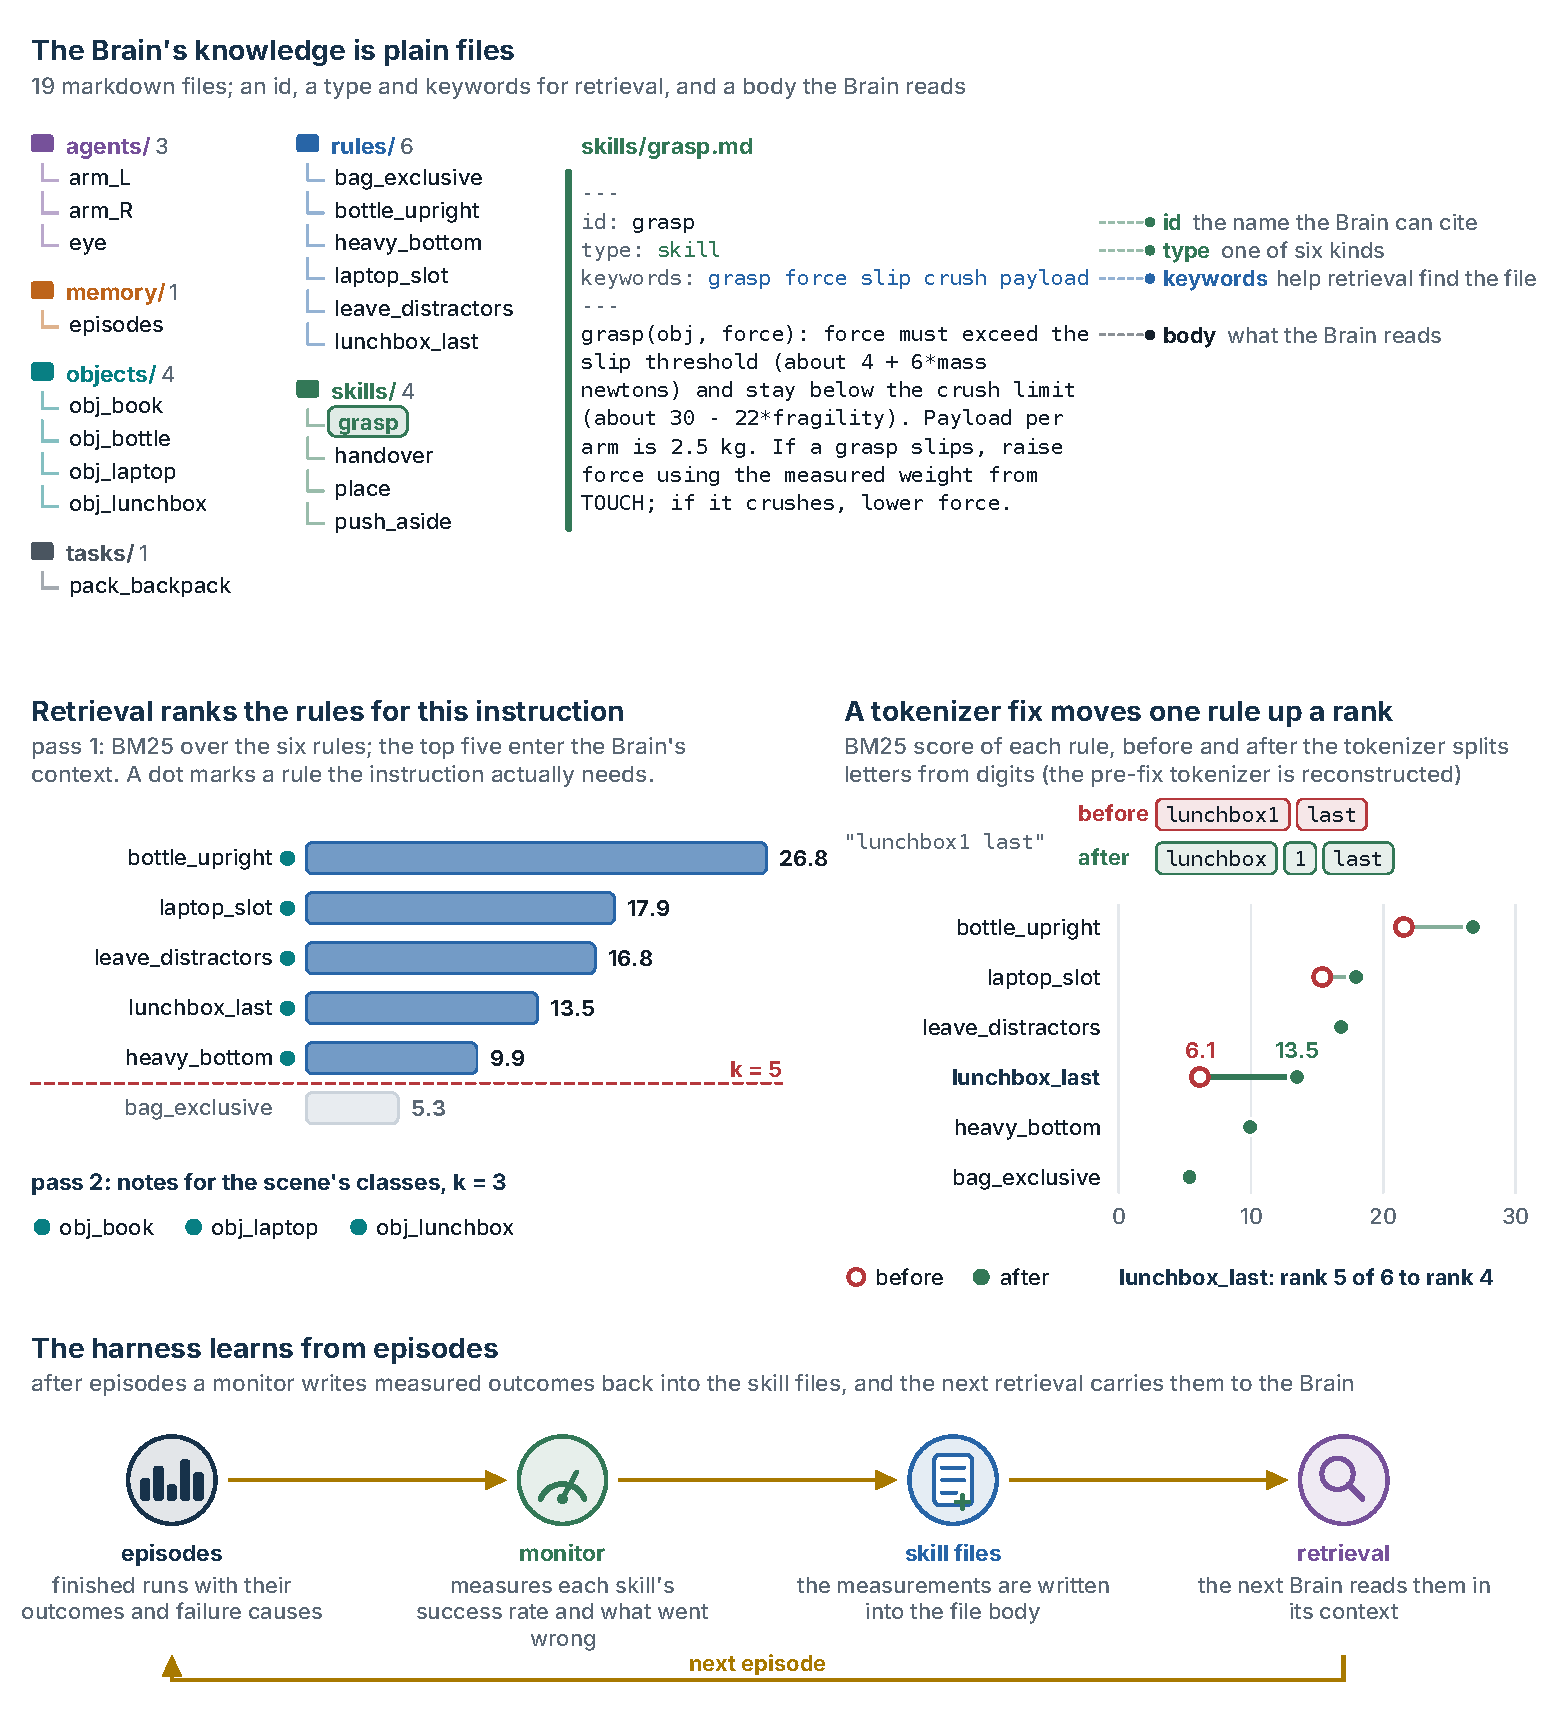
\includegraphics[width=\textwidth]{fig_harness}
\caption{\textbf{The harness.} (a)~The \nHarnessFiles{} markdown files by type. (b)~Two-pass BM25 retrieval into the Brain's context, with a monitor that writes measured outcomes back to the skill files (dashed: runs after episodes). (c)~Tokenization of the string ``lunchbox1 last'' before and after the fix, and the BM25 score of every rule for the recorded instruction. The pre-fix tokenizer is our reconstruction.}
\label{fig:harness}
\end{figure*}

\subsection{Planning with tools and verification}\label{sec:tools}
The Brain can be a plain planner or a tool-using one (\cref{fig:tools}).
The tool-using Brain has \nTools{} tools: \texttt{check\_rule}, \texttt{query\_scene}, \texttt{look}, \texttt{dry\_run} and \texttt{submit\_plan}.
\texttt{dry\_run} executes a draft plan deterministically in the symbolic world and returns the rule violations and failed tasks, which is the evidence the Brain revises against; the prompt asks it to dry-run before submitting, it has at most six turns, and replying with a bare plan also commits.
Independently of the tools, the loop can verify a plan before any arm moves: not at all, with a static feasibility check, or with a full dry run; a rejected plan is returned with the reasons for up to two retries.
We test the verifier against a flaky-planner fixture in appendix~F.

\begin{figure*}[tbp]
\centering
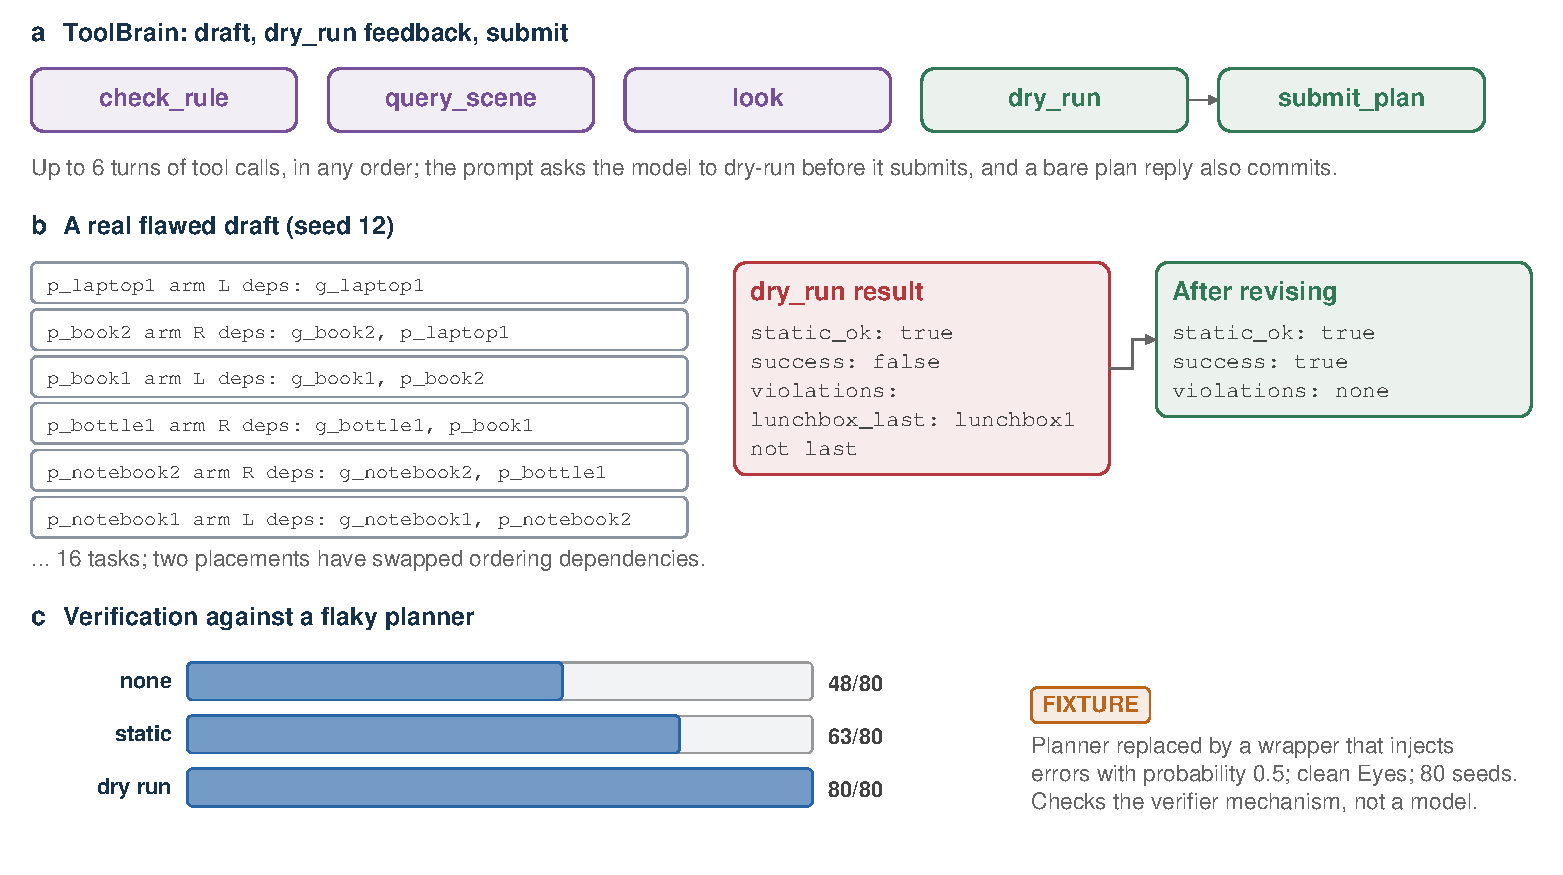
\includegraphics[width=\textwidth]{fig_tools}
\caption{\textbf{Tools and verification.} (a)~The five tools of the tool-using Brain. (b)~A recorded flawed draft (seed \toolSeed{}, two placements with swapped ordering dependencies) and the \texttt{dry\_run} feedback it receives; the revised plan passes. (c)~Verification against a planner replaced by a wrapper that injects errors with probability 0.5 (fixture, 80 seeds): a check of the verifier, not of a model.}
\label{fig:tools}
\end{figure*}

\subsection{The control loop}\label{sec:loop}
An episode runs as in \cref{fig:loop}.
The Eyes report a scene; an optional \emph{probe} has the Arms weigh every item and overrides the Eye mass guesses with measurements.
The Brain plans and the verifier checks.
If a requested item is missing from the scene, the Brain asks the Eyes to \textsc{look} again and replans.
In each round the scheduler gives each Arm its head task, with exclusive access to the bag.
When an Arm touches an item whose measured weight differs from the Eye's report by more than 20\%, it sends a \textsc{challenge}, the scene is corrected and the remaining placements are replanned once.
A human may \textsc{amend} the instruction mid-episode, which forces a replan.
A failed skill climbs a recovery ladder: retry, alternate parameters, retreat, reassign to the other Arm, replan, abort.
At the end the checker of \cref{sec:success} scores the bag and attributes fatal failures.

\begin{figure*}[tbp]
\centering
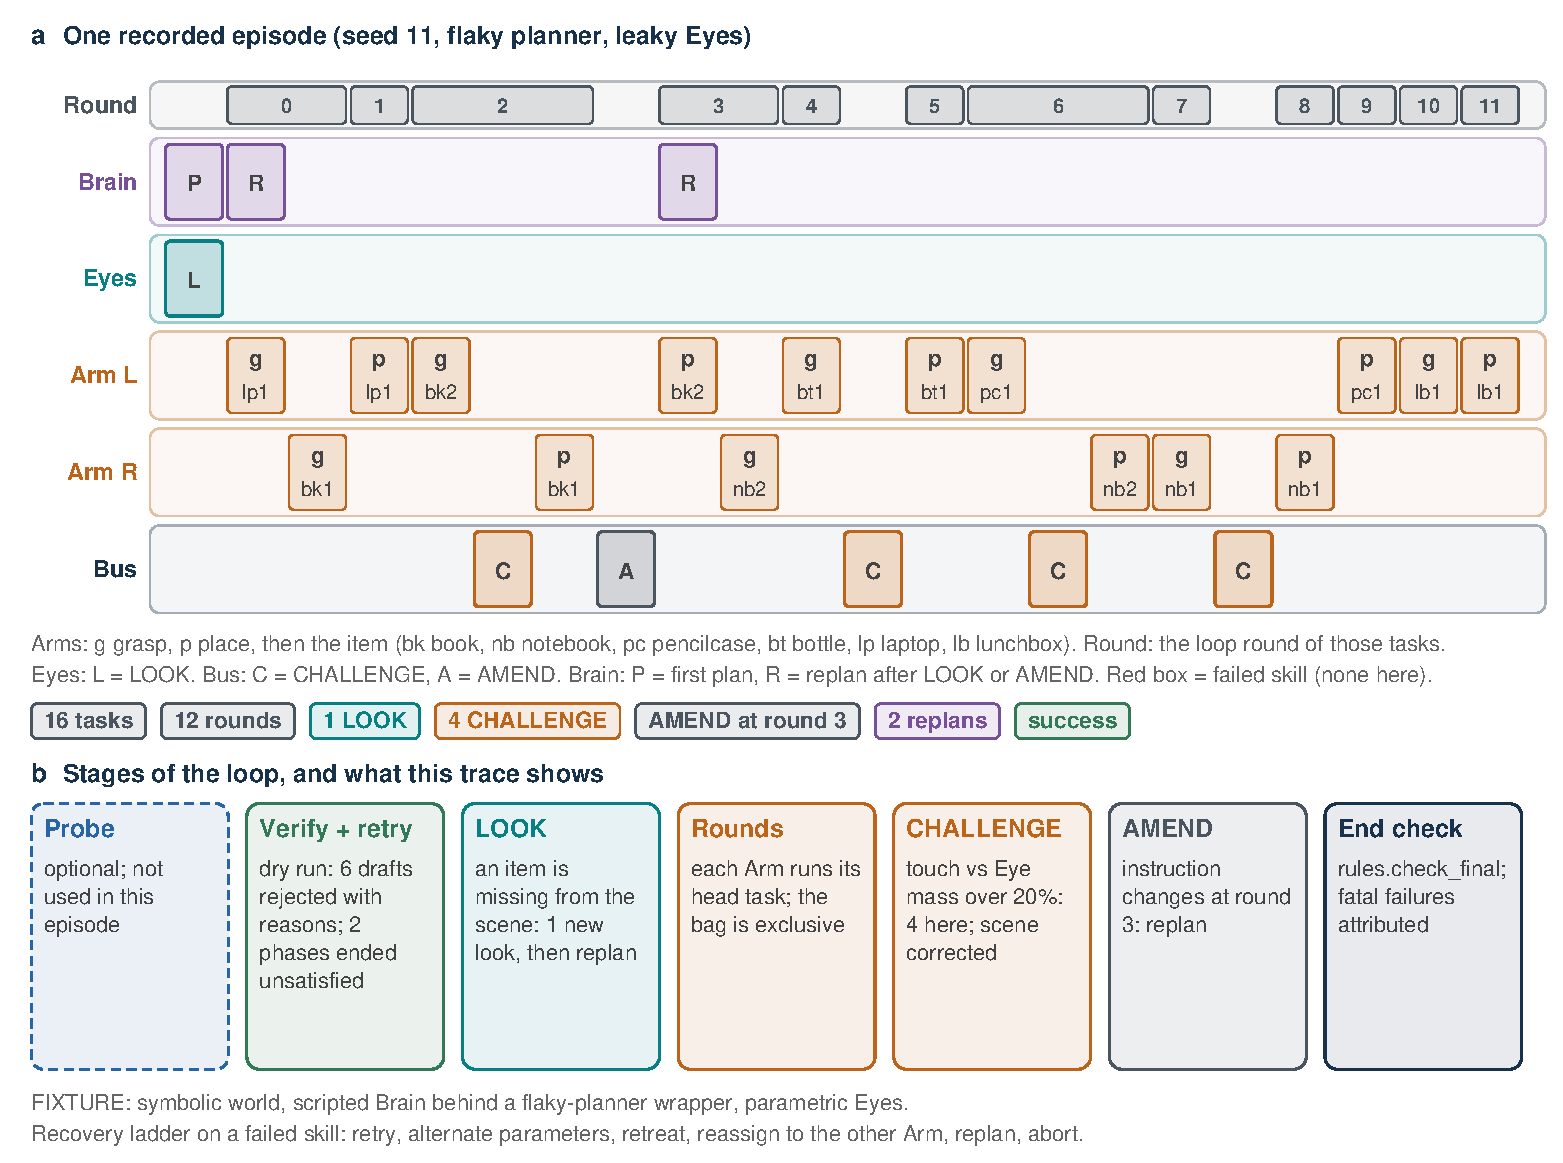
\includegraphics[width=\textwidth]{fig_loop}
\caption{\textbf{One recorded episode through the loop} (seed \loopSeed{}, flaky planner, leaky Eyes; fixture). (a)~The \loopTasks{} executed tasks by arm in time order, with the loop round of each, the \loopLooks{} look, \loopChal{} challenges, the amendment at round \loopAmendRound{} and the replans (\loopReplans{}); the episode takes \loopRounds{} rounds and succeeds. (b)~The stages of the loop and what this trace shows of each, including the planner's \loopRej{} rejected drafts; the probe is not used here.}
\label{fig:loop}
\end{figure*}

\subsection{Success, forces and attribution}\label{sec:success}
One function, \texttt{rules.check\_final}, defines success in every world: every requested item is packed, no rule is violated and nothing is crushed; the score is the valid-item fraction minus 0.15 per violation, 0.3 per crushed item and 0.01 per replan.
In the symbolic world a grasp slips when its force is below $(4+6m)/f$ newtons for mass $m$ and friction $f$, and crushes when it exceeds $30-22\,\phi$ newtons for fragility $\phi$.
Failures are attributed by rules: a slip or crush is charged to the Eye when the reported mass or fragility was off by more than 15\%, otherwise to the Arm; a rule violation is charged to the agent whose report or plan produced it.
These are heuristics; \cref{tab:attribution} is the hand-labelled check we owe the reader.

\subsection{Learning signals}\label{sec:signals}
\Cref{fig:signals} lists what trains what.
Each Eye is fine-tuned with LoRA on rendered images with scene targets and then improved by rejection sampling: $K=8$ reports per image, keeping the best by field accuracy or by counterfactual credit.
The Brain is fine-tuned on teacher plans that were validated by closed-loop success and then optimized with GRPO using a plan-level reward $R = 0.1\,r_{\text{format}} + 0.2\,r_{\text{feasible}} + 0.6\,r_{\text{rules}} + 0.1\,r_{\text{length}}$, optionally plus a closed-loop rollout term; the components are defined in \cref{fig:signals}.
The Arms are a small transformer trained by distillation of scripted differential-IK demonstrations with a flow-matching action head: with $x_t=(1-t)x_0+t\,x_1$, noise $x_0$ and action chunk $x_1$, the network predicts $x_1-x_0$; sampling uses eight Euler steps, a chunk of 16 actions of dimension 8, and executes the first four before replanning.
There is no learned stop signal, so a skill ends by a scripted completion test.

\paragraph{Counterfactual Eye credit.}
For an episode with score $R(\text{real})$, replace Eye $i$'s report by a replacement $r$ (empty, degraded or the oracle truth, optionally for one field only) and replay with the same keyed random draws, giving $R(i,r)$.
The credit is $C(i,r)=R(\text{real})-R(i,r)$, so a positive credit means the Eye helped relative to the replacement; the \emph{oracle gain} $G=R(\text{oracle})-R(\text{real})=-C(i,\text{oracle})$ is what a perfect Eye would have added.
All random draws are keyed by (seed, arm, skill, object, attempt), so replays share common random numbers.
The estimate has two caveats: it is a team counterfactual and is not additive across redundant Eyes, and with a Brain that adapts to the replaced report it measures the adapted team, not the original plan.
\Cref{fig:credit}a shows one recorded case: a perfect Eye~A would recover \credGain{} of a score of \credBase{}, all of it in the mass field.

\paragraph{Team hindsight relabeling.}
A finished episode is relabeled with what the team achieved: the instruction is rewritten to the rules that held, and the executed plan becomes the target.
The record is admitted only if replaying the executed plan from the initial state satisfies the relabeled instruction.
In \cref{fig:credit}b the failed episode of \cref{fig:mechanism} is relabeled by dropping \hindDropped{}, and its \hindTasks{}-task plan passes the replay check.
The relabeled instruction is weaker than the original, so relabeled data teaches obedience to what was achievable and must be mixed with unrelabeled data; the mixing ratio is a pending ablation.

\begin{figure}[tbp]
\centering
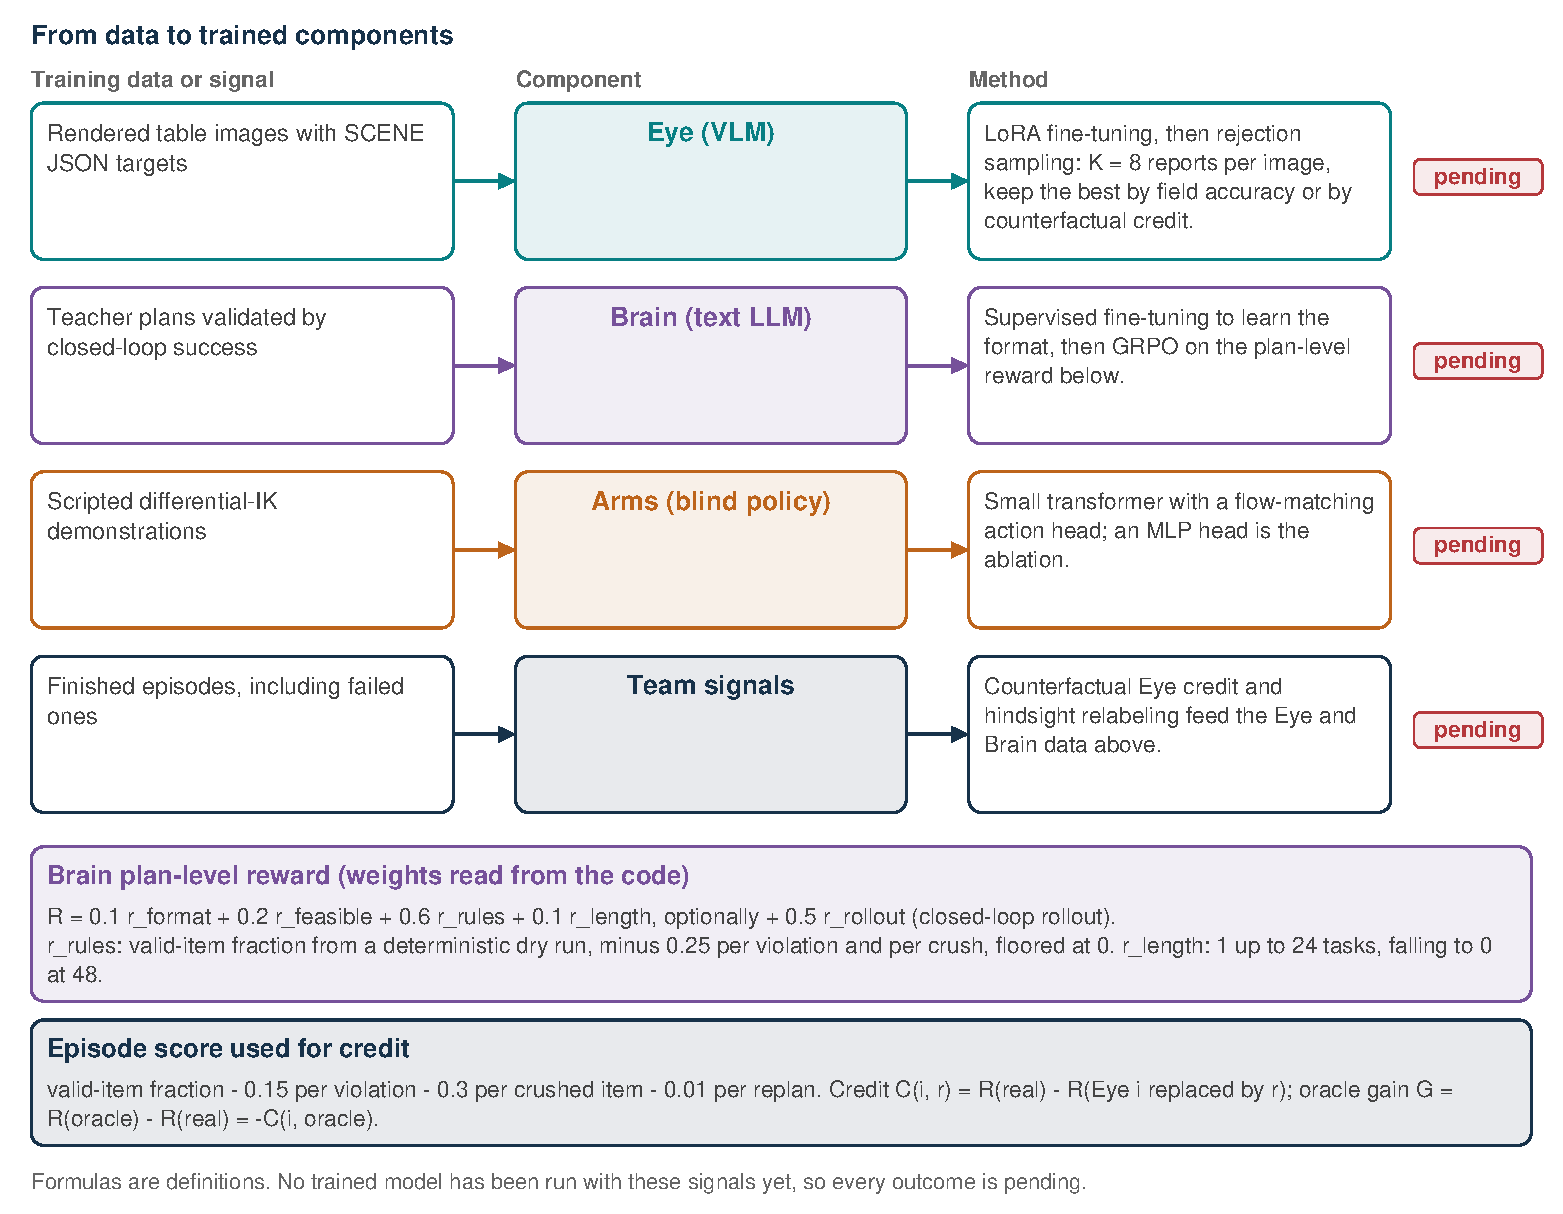
\includegraphics[width=\columnwidth]{fig_signals}
\caption{\textbf{Learning signals.} From training data through component to method, then the plan-level reward read from the code and the episode score used for credit. No trained model has been run with these signals, so all outcomes are pending.}
\label{fig:signals}
\end{figure}

\begin{figure*}[tbp]
\centering
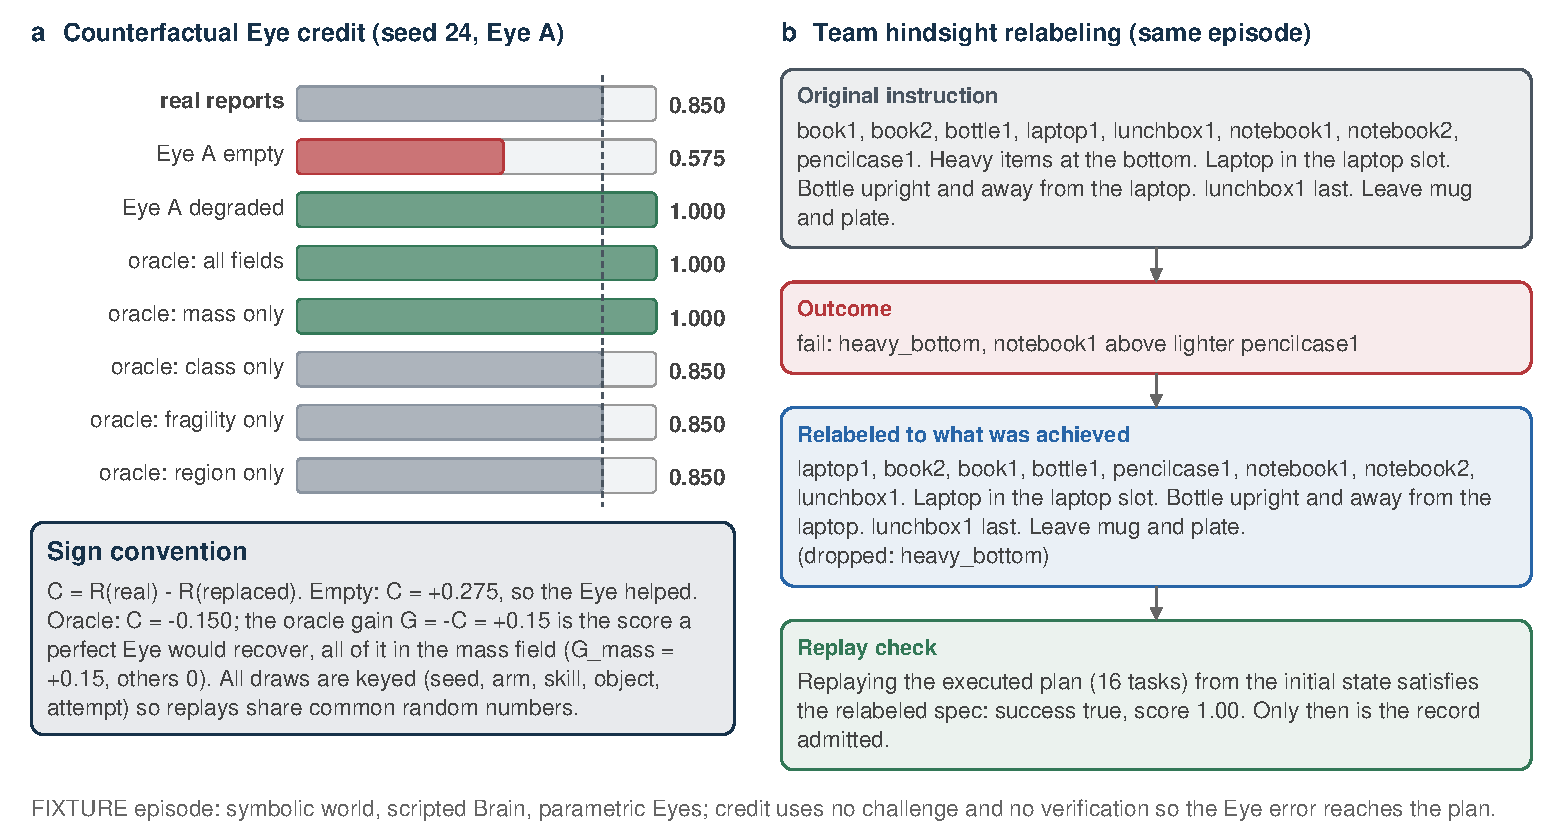
\includegraphics[width=\textwidth]{fig_credit}
\caption{\textbf{Two team-level signals on the episode of \cref{fig:mechanism}.} (a)~Counterfactual credit for Eye~A: replacing its report changes the episode score; the dashed line is the real score (\credBase{}) and an empty report would score \credEmpty{}. (b)~Hindsight relabeling: the failed episode is rewritten to what it achieved and admitted only after a replay check. Fixture episode (no challenge, no verification, so the Eye error reaches the plan).}
\label{fig:credit}
\end{figure*}

\subsection{One success definition across three worlds}\label{sec:bridge}
The same team runs in three worlds (\cref{fig:bridge}): the symbolic world, in which the loop is developed; a pose-level fake simulator that takes poses, maps them to regions and compartments through a bridge and reproduces the symbolic world's loop outcomes in tests; and Isaac Lab, where skill outcomes (success, slip, crush, out of reach, wrong slot, no space, locked, overload, not holding, hand full) are derived from the state before and after a skill.
Because \texttt{rules.check\_final} scores all three, the difference between a plan that is valid in the symbolic world and one that succeeds under physics can be measured instead of assumed.
The pose-level test validates the integration, not the physics.

\begin{figure*}[tbp]
\centering
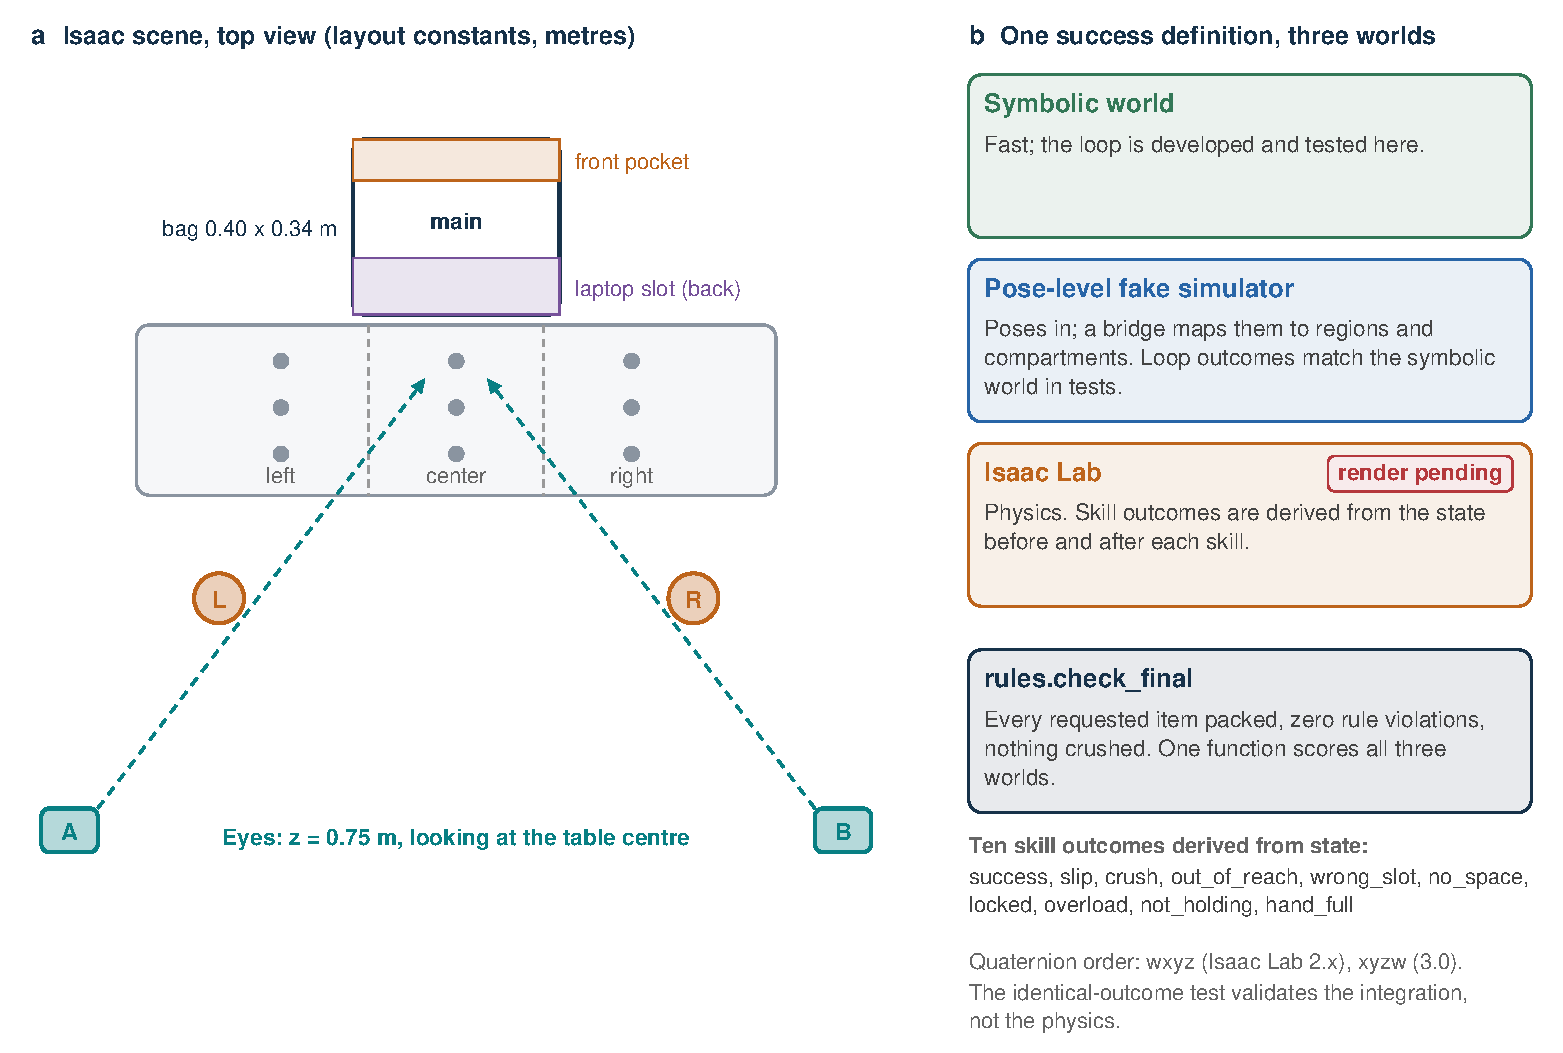
\includegraphics[width=\textwidth]{fig_bridge}
\caption{\textbf{The Isaac scene and the shared checker.} (a)~Top view from the layout constants: table zones, bag compartments, arm bases and camera positions. (b)~One success function scores three worlds. The Isaac render is pending.}
\label{fig:bridge}
\end{figure*}
